\chapter{实验数据分析}\label{chap:Epxeriment}

\section{实验环境}


\section{调试环境}

本章节首先展示微译器在X86上SPEC 2017上的翻译运行结果,然后介绍RISCV在CoreMark测试集上的运行效果。

\section{微译器在X86上的翻译运行结果}

图\ref{img:ucache_ipc}展示了微译器在X86上SPEC 2017上的翻译运行结果,相对于未修改过的X86指令缓存模式进行了归一化。
可以看到,微译器在SPEC 2017上的性能接近于原生运行,平均性能为92.3\%,并且一大半的浮点型测试集的性能损失在1\%以内。

\begin{figure}[h]
  \centering
  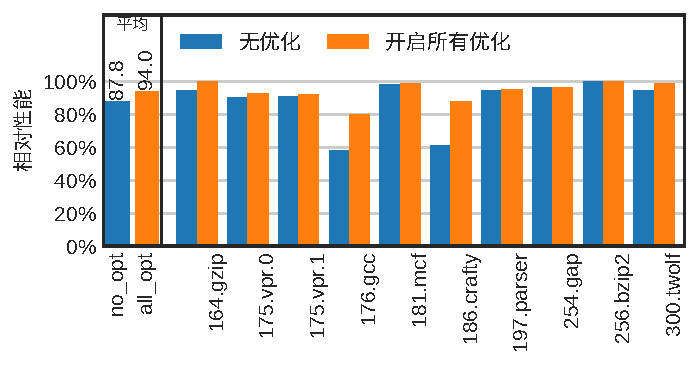
\includegraphics[width=1\linewidth]{./plot/ucache_ipc.pdf}
  \caption{微译器运行SPEC CPU 2017的性能,相对于未修改过的X86指令缓存模式进行了归一化。}
  \label{img:ucache_ipc}
\end{figure}

图\ref{img:new_cache_miss}展示了微译器在X86上SPEC 2017上的每千条指令的未命中次数(MPKI),
根据计算,每千条指令的未命中次数和性能之间的皮尔森相关系数为-0.93,说明未命中次数和性能之间存在很强的负相关性。
这也说明了微译器的性能主要受到了未命中次数的影响。

\begin{figure}[h]
  \centering
  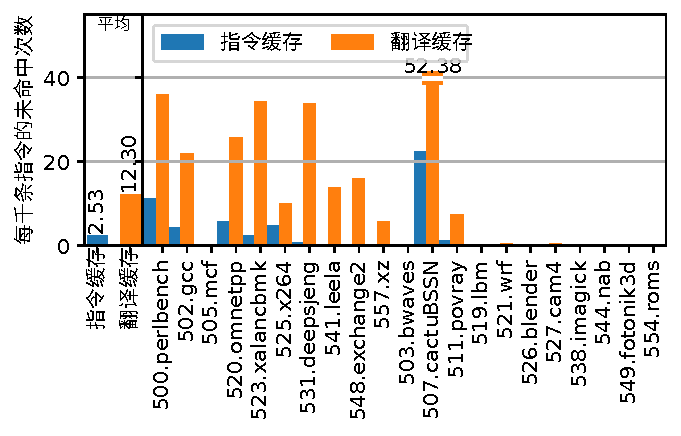
\includegraphics[width=1\linewidth]{./plot/new_cache_miss.pdf}
  \caption{微译器运行SPEC CPU 2017的每千条指令的未命中次数。}
  \label{img:new_cache_miss}
\end{figure}

\section{微译器在CoreMark测试集上的运行结果}

\begin{table}[]
  \centering
  \caption{
    微译器运行CoreMark测试集的性能对比。
  }
  \label{tab:coremark}
  \begin{tabular}{llll}
  \rowcolor[HTML]{FFCE93} 
               & x86\_raw & x86\_ucache & riscv\_ucache \\
  Insts        & 34655642 & 34655642    & 35899262      \\
  Cycles       & 26220774 & 26301941    & 28797485      \\
  IPC          & 1.321686 & 1.317608    & 1.246611      \\
  IPC/IPC\_raw & 100\%    & 99.69\%     & 94.32\%      
  \end{tabular}
  \end{table}

我们在X86上运行了CoreMark测试集,相对于普通的ICache配置项,也就是没有任何修改的运行X86程序,
我们的微译器在翻译运行的性能为99\%,对应的每千条指令的未命中次数为0.9,也符合上述规律,
这主要在于程序的取指行为,CoreMark程序中主要为核心循环计算,时间局部性和空间局部性都很好,因此未命中次数较少,性能也较好。
即便经过微译器的预翻译文件膨胀,也能够在X86上保持较好的性能。

我们在RISCV上运行了CoreMark测试集,得到了性能为94\%,对应的每千条指令的未命中次数为1.1,也符合上述规律。

RISCV 相对于X86的CoreMark 还有一定的性能差距,主要由于还没有添加硬件返回栈支持,导致对于函数调用的支持不够完善,因此性能有所下降。

同时RISCV目前对于压缩指令支持还不够完善,导致翻译出来的微码编码较长,导致AOT文件相对更大,也会导致性能下降。


\section{微译器在RISCV上的翻译运行结果}
由于Gem5的模拟器的性能开销较大,我们选择了SPEC CPU 2000 test测试集作为测试基准。
SPEC CPU 2000 test测试集包括了12个整数测试程序和14个浮点测试程序,是一个较为完备的测试集。
目前已经成功运行了8个整数测试程序,剩下的整数测试程序由于指令翻译的问题暂时无法运行,目前还在修复中,浮点测试程序还没有测试。

如图\ref{img:ipc}所示,我们的微译器在运行SPEC CPU 2000 test测试集时(这里只关注RISCV程序),总共有三个测试配置,分别为:
\begin{itemize}
  \item 不带微码缓存:CPU直接从内存中取指,没有经过内存层次结构,没有延迟,只是为了对比理想值。
  \item 带有微码缓存:CPU经过内存层次结构,经过L2Cache和微码缓存(相当于L1ICache),有取值延迟,有大量冷缺失。
  \item 带有微码缓存并有优化:在上一个配置基础上,加上了两个微码缓存放松条件,还加上了微码压缩机制,让一行微码行中存储微码指令数目变多了,减少缺失率。
\end{itemize}
注意这三个配置都是运行RISCV程序的测试,运行X86程序的对比测试会在之后进行。

\begin{figure}[h]
  \centering
  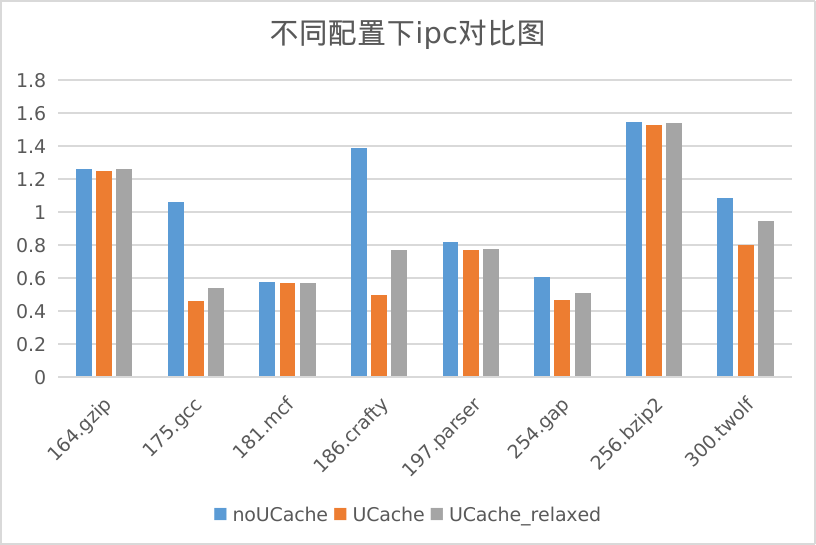
\includegraphics[width=0.8\linewidth]{./plot/ipc.png}
  \caption{ipc对比图。}
  \label{img:ipc}
\end{figure}

如图\ref{img:ipc}所示,我们的微译器在运行SPEC CPU 2000 test测试集时,性能表现如下:
对于gcc和crafty两个测试程序,我们的微译器的性能表现在加上微码缓存后,性能下降了约50\%;
这是由于这两个测试程序代码循环较少,时间局部性较差,导致了大量的冷缺失;
这应该需要加上更多的优化手段,例如添加微码缓存预取机制,减少冷缺失。
而对于其他的几个测试程序,性能大多在90\%以上,说明这些程序的时间局部性较好,性能下降较少,微译器的性能表现较好。

如图\ref{img:MPKI}所示,我们的微译器在运行SPEC CPU 2000 test测试集时,每千条指令的未命中次数(MPKI)表现如下:
经过计算,未命中次数和性能之间的皮尔森相关系数为-0.91,说明未命中次数和性能之间存在很强的负相关性。目前的性能下降主要受到了未命中次数的影响。

\begin{figure}[h]
  \centering
  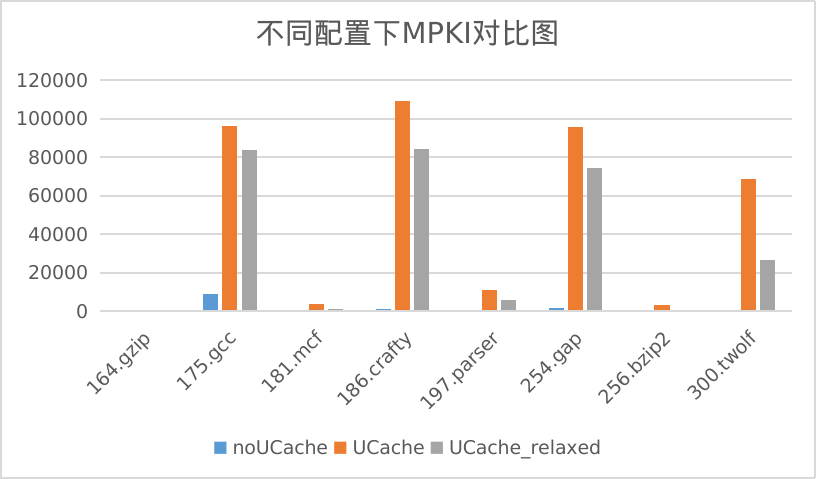
\includegraphics[width=0.8\linewidth]{./plot/MPKI.png}
  \caption{MPKI对比图。}
  \label{img:MPKI}
\end{figure}
